\documentclass{article}
\usepackage[toc,page]{appendix}
\usepackage{blindtext}
\usepackage{titlesec}
\usepackage{graphicx} % Required for inserting images
\usepackage{float}
\usepackage[ddmmyyyy,hhmmss]{datetime}
\usepackage{listings}% http://ctan.org/pkg/listings
\usepackage{amsmath}
\usepackage{hyperref}
\usepackage{biblatex}
\usepackage[dvipsnames]{xcolor}
\usepackage{parskip}
\usepackage[most]{tcolorbox}
\usepackage{lineno}


\colorlet{myfigurecolor}{teal!90!blue}
\colorlet{myfigurecolorback}{myfigurecolor!10!white}
\colorlet{myexamplecolor}{cyan!40!green}
\colorlet{myexamplecolorback}{myexamplecolor!10!white}
\colorlet{myinlinecolorback}{gray!10!white}
\tcbset{
    enhanced,
    colback=myfigurecolor!5!white,
    boxrule=0.1pt,
    colframe=myfigurecolor,
    fonttitle=\small\bfseries,
    fontupper=\small,
    center title
}

\newtcolorbox[blend into=figures]{myfigure}[2]{
    colback=myfigurecolorback, 
    colframe=myfigurecolor, 
    title={#1},
    label={#2},
    center,
    fontupper=\footnotesize
}

\newtcolorbox[auto counter]{example}[2]{
    colback=myexamplecolorback, 
    colframe=myexamplecolor, 
    title=Example \thetcbcounter: #1, 
    label={#2},
    center,
    breakable,
    fontupper=\footnotesize
}

\addbibresource{references/ref.bib}

\hypersetup{
    colorlinks=true,
    linkcolor=cyan,
    citecolor=cyan,
    filecolor=magenta,      
    urlcolor=cyan,
    pdftitle={Overleaf Example},
    pdfpagemode=FullScreen
}

\definecolor{codegreen}{rgb}{0,0.6,0}
\definecolor{codegray}{rgb}{0.5,0.5,0.5}
\definecolor{codepurple}{rgb}{0.58,0,0.82}
\definecolor{backcolour}{rgb}{0.95,0.95,0.92}

\lstdefinelanguage{elm}
{
  % List of keywords
  morekeywords={
    alias,
    as,
    case,
    else,
    exposing,
    if,
    import,
    in,
    let,
    module,
    of,
    port,
    then,
    type,
    where
  },
  sensitive=true, % Keywords are case-sensitive
  morecomment=[s]{\{-}{-\}}, % s is for start and end delimiter
  morecomment=[l]{--},
  morestring=[b]" % Defines that strings are enclosed in double quotes
}


\lstdefinestyle{inline}{
    basicstyle=\small\ttfamily, % Global Code Style
    captionpos=b, % Position of the Caption (t for top, b for bottom)
    extendedchars=true, % Allows 256 instead of 128 ASCII characters
    tabsize=2, % Number of spaces indented when discovering a tab 
    columns=fixed, % Make all characters equal width
    keepspaces=true, % Does not ignore spaces to fit width, convert tabs to spaces
    breaklines=true, % Wrap lines if they don't fit
    showstringspaces=false, % Lets spaces in strings appear as real spaces
    mathescape=true, % Enable math escape
    commentstyle=\color{codegreen},
    keywordstyle=\color{magenta},
    numberstyle=\tiny\color{codegray},
    stringstyle=\color{codepurple},
    backgroundcolor=\color{myinlinecolorback},   
}

\definecolor{elm-orange}{RGB}{240,173,0}
\definecolor{elm-gray}{RGB}{149,149,138}
\definecolor{elm-blue}{RGB}{0,168,198}

\lstdefinestyle{mystyle}{
    backgroundcolor=\color{myexamplecolorback},   
    commentstyle=\color{codegreen},
    keywordstyle=\color{magenta},
    numberstyle=\tiny\color{codegray},
    stringstyle=\color{codepurple},
    basicstyle=\ttfamily\footnotesize,
    breakatwhitespace=false,         
    breaklines=true,                 
    captionpos=b,                    
    keepspaces=true,                 
    numbers=left,                    
    numbersep=5pt,                  
    showspaces=false,                
    showstringspaces=false,
    showtabs=false,                  
    tabsize=2
}

\newcommand{\mybox}[3]{\begin{center}
\begin{myfigure}{#1}{#2}
\begin{varwidth}{\textwidth}#3\end{varwidth}
\end{myfigure}
\end{center}}

\lstset{style=mystyle}

\setlength{\parindent}{0pt} % No indentation
\title{Cursors in sub-sub-trees}
\date{}
\author{}

\begin{document}
\maketitle
% \linenumbers
The syntax of well-formed trees is given by:

\begin{enumerate}
    \item The sorts $\dot{\mathcal{S}} = \hat{\mathcal{S}} \cup \{ \dot{s} \}_{s \in \mathcal{S}}$
    \item The family of operators $\dot{\mathcal{O}} = \hat{\mathcal{O}}$ extended with an operator of arity $(\hat{s})\dot{s}$ for every $\hat{s} \in \hat{\mathcal{S}}$
    \item For every operator $\hat{o} \in \hat{\mathcal{O}}$ of arity $(\vec{\hat{s}}_1.\hat{s}_1,...,\vec{\hat{s}}_n.\hat{s}_n)\hat{s}$ and for every $1 \leq i \leq n$ the operator $\dot{o}_i$ of arity $(\vec{\hat{s}}_1.\hat{s}_1,...,\vec{\hat{s}}_i.\hat{s}_i,...,\vec{\hat{s}}_n.\hat{s}_n)\dot{s}$ is added to $\dot{\mathcal{O}}$
    \item The family of variables $\dot{\mathcal{X}} = \hat{\mathcal{X}}$
\end{enumerate}

Where $\hat{\mathcal{S}}$ is the set of cursorless sorts and $\hat{\mathcal{O}}$ is the family of cursorless operators.

This definition of well-formed trees only allow the cursor to encapsulate either the root of a cursorless abt, or one of its first children. In other words, this does not allow having a cursor in a grandchild or deeper. See figure \ref{fig:ex} for an example of a tree that is not deemed well-formed, since the cursor does not encapsulate the root or one of the first children.

\begin{figure}[H]
    \centering
    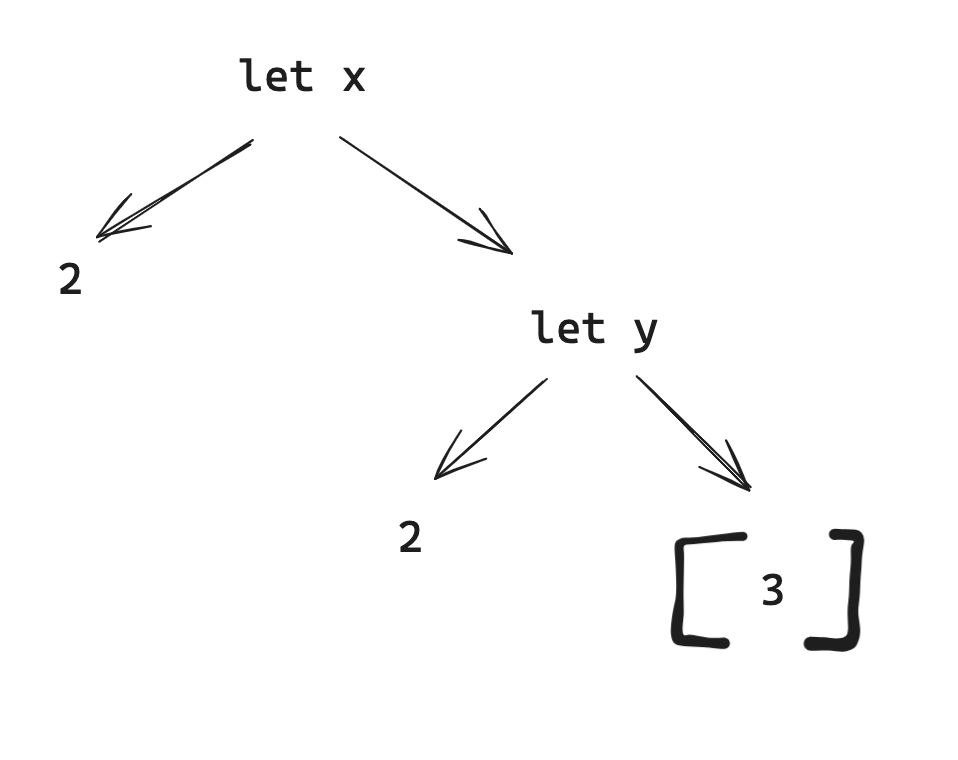
\includegraphics[scale=0.3]{img/not-well-formed-example.png}
    \caption{Disallowed cursor placement wrt. the well-formed tree definition}
    \label{fig:ex}
\end{figure}

Another thing that might be related and that also confuses me is the \texttt{WellFormedAst} type in the KU bachelor project being defined as a type alias for the \texttt{C} type, which is the cursor context:

\begin{lstlisting}[style=inline,language=elm]
{-| Represents an AST cursor context.
-}
type C
    = Cursor Ast
    | CApp1 C Ast
    | CApp2 Ast C
    | CLambda Var.Id ATyp C
    | CLet1 Var.Id ATyp C Ast
    | CLet2 Var.Id ATyp Ast C
    | CLetrec1 Var.Id ATyp C Ast
    | CLetrec2 Var.Id ATyp Ast C
    | CPatterns1 L C Ast
    | CPatterns2 L Ast C
    | CPattern L C
    | CBreak C


{-| An alias for an AST cursor context.
-}
type alias WellFormedAst =
    C
\end{lstlisting}

Although, this might 

\printbibliography

\end{document}